\subsection{Електроненн контролер на скоростта за безчеткови постояннотокови мотори (ESC)}

Използван е контролер на скоростта за безчеткови постояннотокови мотори \textit{Plush 40amp Speed Controller} (\autoref{fig:esc_hardware}) на \textit{TURNIGY}.
Контролерът може да черпи максимум \(40A\) ток за продължително време,
както и максимален моментен ток \(55A\) (\(>10s\)) \cite{user_manual_esc}.

Използвана е настройка за Li-Po батерия,
спирачка-включена,
опция за намаляване на мощността,
средна граница на намаляване на мощността,
нормално стартиране,
средно време за реакция.
Посоката на въртене не е софтуерно настройваема.
За смяна на посоката на въртене се разменят които и да е два от изходите към безчетковия мотор.
Това променя последователността на сигналите към отделните намотки и посоката на въртене се обръща.

Опциите за насторйка и процедурата са описани в \cite{user_manual_esc}.
Важно е да се отбележи, че моторите се инициализират след около 6 секунди,
при възможно най-ниска стойност на управляващия сигнал.
Управляващият сигнал е с честота 50Hz и е ШИМ със запълване между (\(1000\pm50 \to 2000\pm50 \mu s\)).

\begin{figure}[htpb!]
    \centering
    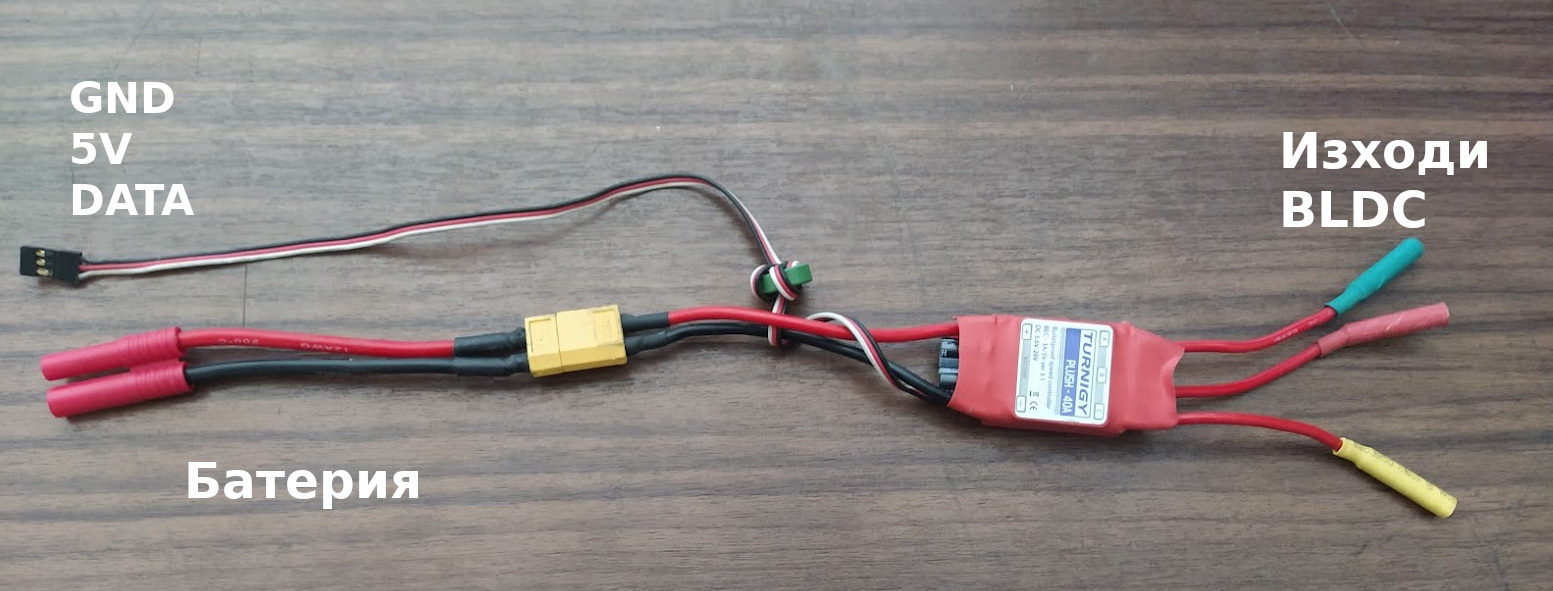
\includegraphics[width=0.7\textwidth]{esc_hardware}
    \caption{ESC с анотация на изходите и входовете}
    \label{fig:esc_hardware}
\end{figure}

\FloatBarrier
